%
% The first command in your LaTeX source must be the \documentclass command.
\documentclass[sigchi]{acmart}
\usepackage{cancel}
\usepackage{graphicx}
\usepackage{adjustbox}
\usepackage{ulem}
\usepackage{placeins}
\usepackage{graphicx}
\usepackage{subcaption}
\usepackage{afterpage}
\usepackage{amsmath}
\usepackage{float}
\usepackage{fancyhdr}
\usepackage{wrapfig}
\usepackage{adjustbox}
\usepackage{tabularx}
\pagestyle{fancy}
\fancyhf{}
\rfoot{\thepage}

%
% defining the \BibTeX command - from Oren Patashnik's original BibTeX documentation.
\def\BibTeX{{\rm B\kern-.05em{\sc i\kern-.025em b}\kern-.08emT\kern-.1667em\lower.7ex\hbox{E}\kern-.125emX}}
    
% Rights management information. 
% This information is sent to you when you complete the rights form.
% These commands have SAMPLE values in them; it is your responsibility as an author to replace
% the commands and values with those provided to you when you complete the rights form.
%
% These commands are for a PROCEEDINGS abstract or paper.
\copyrightyear{2023}
\acmYear{2023}
\setcopyright{acmlicensed}
\acmConference[SNA '23]{Social Network Analysis '23}{2022/23}{University of Pisa, Italy}
\acmBooktitle{Social Network Analysis '23}
\acmPrice{0.00}



% end of the preamble, start of the body of the document source.
\begin{document}

%
% The "title" command has an optional parameter, allowing the author to define a "short title" to be used in page headers.
\title{Topic Modeling of ChatGPT users on Reddit}

%
% The "author" command and its associated commands are used to define the authors and their affiliations.
% Of note is the shared affiliation of the first two authors, and the "authornote" and "authornotemark" commands
% used to denote shared contribution to the research.
\author{Claudio De Martino}
\email{c.demartino1@studenti.unipi.it}
\affiliation{%
  \institution{Student ID: 560934}
}

\author{Giuliano Galloppi}
\email{g.galloppi@studenti.unipi.it}
\affiliation{%
  \institution{Student ID: 646443}
}

\author{Clara Lavorati}
\email{c.lavorati@studenti.unipi.it}
\affiliation{%
  \institution{Student ID: 565091}
}

\author{Isabel Santucci}
\email{i.santucci@studenti.unipi.it}
\affiliation{%
  \institution{Student ID: 597351}
} 


\renewcommand{\shortauthors}{Topic Modeling of ChatGPT users on Reddit}


% The abstract is a short summary of the work to be presented in the article.
\begin{abstract}
Nowadays, ChatGPT is on everyone's lips. Based on an LLM that uses large neural networks to learn and generate text, it is able to answer questions, provide information, perform specific tasks and participate in conversations. The aim of this project's analysis, using Network Science tools, is to investigate how discussion around ChatGPT takes place among users of the social network Reddit, and which topics these fall under, decreting a majority use in a particular area exploiting some interesting statistics from it. \footnote{
{\bf Project Repository:}\\
\url{https://github.com/sna-unipi/sna-2023-2023_de-mart_gall_lavo_sant}}

\end{abstract}


%
% Keywords. The author(s) should pick words that accurately describe the work being
% presented. Separate the keywords with commas.
\keywords{ChatGPT, AI, Reddit, Topic Modeling, LLM, Social Network Analysis}


%
% This command processes the author and affiliation and title information and builds
% the first part of the formatted document.
\maketitle

\section{Introduction}
  ChatGPT is an artificial intelligence model developed by OpenAI, also called Generative Pre-trained Transformer 3 (GPT-3), designed to understand and generate natural text, enabling interaction with it through written conversations. 

  Transformers are deep learning models that have revolutionised the field of Natural Language Processing (NLP). Introduced in 2017 by Vaswani et al.\cite{vaswani2017attention}, they rely on the 'attention' mechanism to handle sequences of words efficiently and capture long-range relationships. This technology has led to significant improvements in the performance of NLP models. 
  
  It is used nowadays in any field and by anyone as a virtual assistant who can answer your questions, provide any kind of information and even support a conversation. The massive use of chatbots is increasingly evolving into the main subject of discussion today: this is the reason that prompted the group to analyse in more detail the discussion that develops around these tools using the social network `Reddit' \cite{reddit} as the main data source. 
  
  The purpose of this analysis is to investigate the interactions between users, which take place through the exchange of mutual comments, using the knowledge and techniques of Social Network Analysis in order to be able to answer the research question that arose spontaneously to identify in which areas ChatGPT is most discussed; this question was answered by performing a Topic Modeling analysis on the users belonging to the collected data, dated December 2022. The development process of the project initially consisted of a Data Crawling phase from the Social Network, followed by a Pre-processing of the data to make it adaptable to our analysis, after constructing a network graph made of nodes (users) and edges (comments between users). The main metrics that were employed to elaborate the Network Analysis phase include: degree distribution, connected components, path analysis, clustering coefficient, density analysis, centrality analysis. These were then compared with ER and BA graphs constructed with equal numbers of nodes. In the Data Analysis and Network Manipulation phase instead, Community Detection, Spreading, Dynamic Network Analysis and Higher-order Network Analysis tasks were explored, which are detailed in the following sections. Finally, an analysis of the open question discussed earlier on topic modeling with the obtained results is given.
  

\section{Data Collection}
To achieve the goal of this project, we decided to retrieve the data from the Social Network Reddit.\cite{reddit}

\noindent Reddit is a content sharing Social Network that allows users to discuss and share information on a wide range of topics. 
It is based on a system of sub-networks called `subreddits': every subreddit is dedicated to a specific topic to which users can subscribe in order to share content, join discussions and express their preferences using a voting system on posts and comments through the `upvote/downvote' buttons. The algebraic sum of the upvotes and downvotes determines the score of the post or comment.


\subsection{Selected Data Sources}
From a first direct scraping from Reddit using the official APIs through wrappers such as Praw, Pmaw and Psaw, we found an inadequacy of the available scraping methods or the deactivation of the last two. Thus, we decided to use \href{https://academictorrents.com/details/c398a571976c78d346c325bd75c47b82edf6124e/tech&filelist=1}{official data backup} of the social network dating back to December 2022 to avoid inconsistencies of the most recent data. The data was collected from r/ChatGPT subreddit.

\begin{figure}[hbpt]
  \centering
  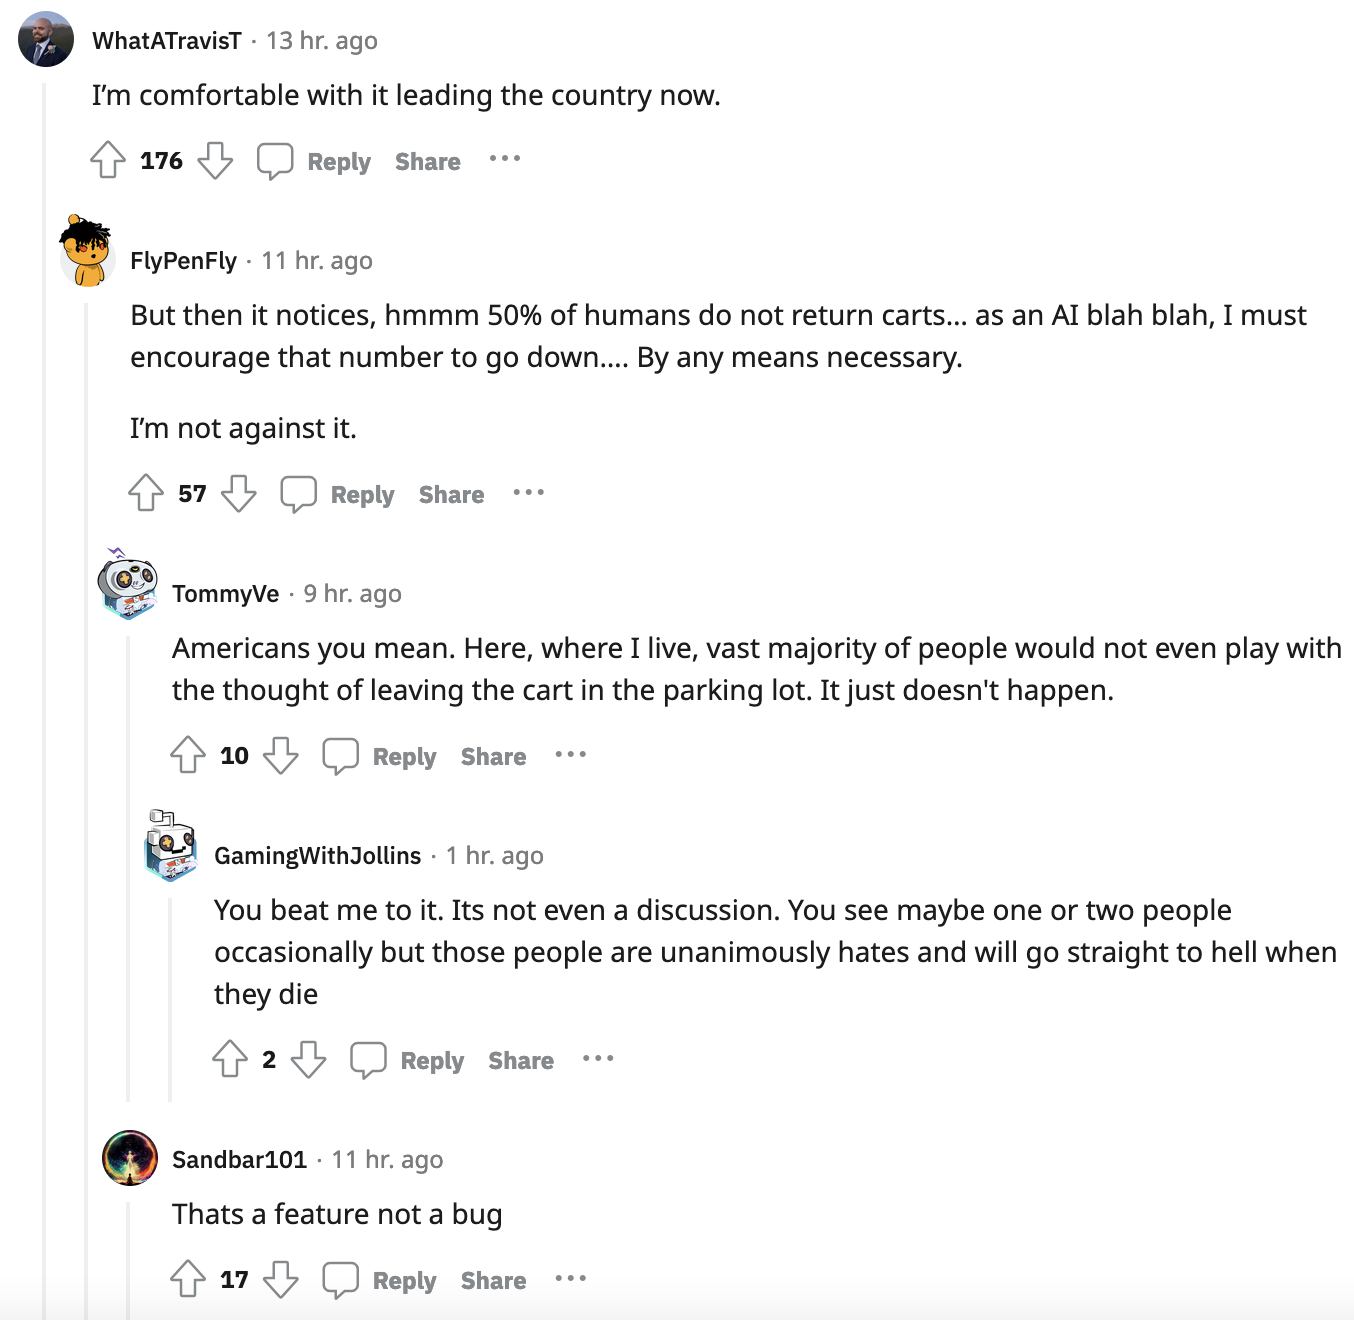
\includegraphics[width=0.8\linewidth]{img/reddit2.png}
  \caption{Exchange of comments in a Reddit post}
  \label{fig:Reddit comments}
\end{figure}

\subsubsection{Crawling Methodology and Assumptions} 
The dataset called `reddit\_comments.csv' contains information about Reddit users and their comments w.r.t. the replies among them, as we can see in the Figure \ref{fig:Reddit comments}. 

It contains 49886 records, which go from 2 December 2022 to 31 December 2022, and 10 attributes.

\noindent The most relevant of them are:
\begin{itemize}
    \item \textit{date}: comment creation date in DD/MM/YYYY format;
    \item \textit{clean\_text}: comment's text;
    \item \textit{author}: unique username of the comment author;
    \item \textit{parent\_author}: unique username of the user who has been replied to by commenting (added later);
    \item \textit{created\_utc}: date the scraped record was added, in UTC format;
    \item \textit{num\_comments}: number of comments, valid only for posts, NaN otherwise;
    \item \textit{score}: comment score obtained by total number of upvotes/downvotes, popularity and discussion engagement;
    \item \textit{type}: type of data collected, post or comment.
\end{itemize}

\noindent The collected data is guided by the assumption the group made for the construction of the graph, i.e. the \textit{nodes} are represented by the users in the dataset, while the \textit{edges} are represented by the exchange of comments between users (i.e. if a user responds to a comment of another user then there is a relationship between them).
The decision was made to represent the graph in an `oriented' manner, motivated by the structure of the replies between users; it returned 13171 nodes, which are the users, and 40948 edges, which are the comment exchanges.

\begin{figure}[hbpt]
  \centering
  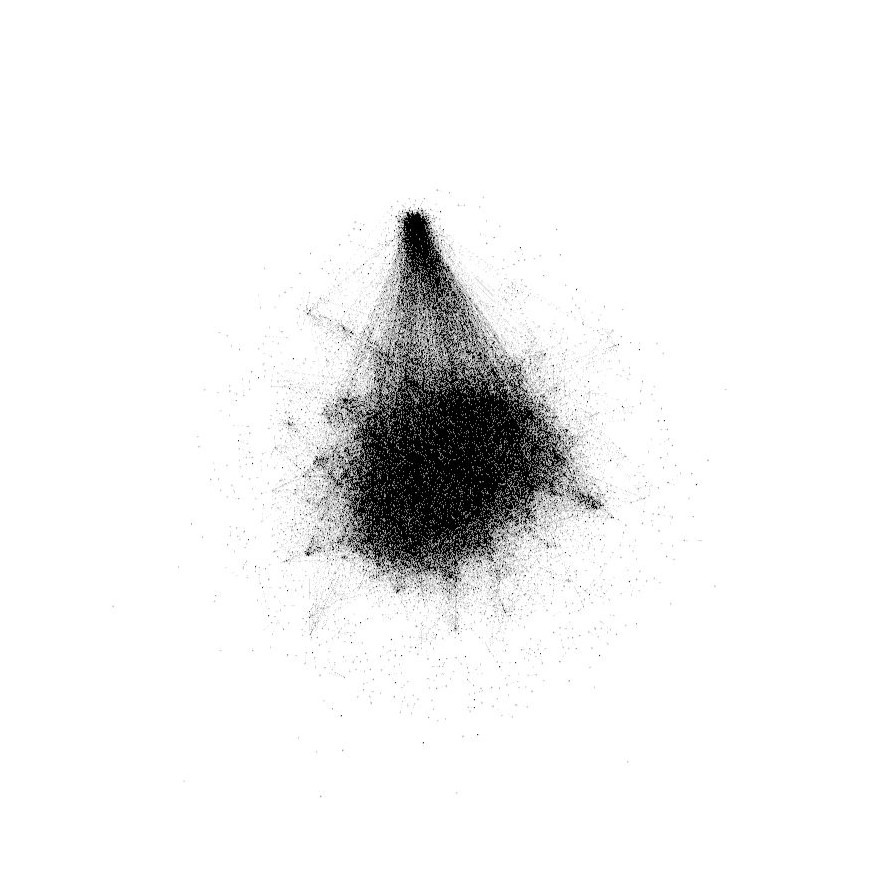
\includegraphics[width=0.8\linewidth]{img/reddit_comments_network.jpg}
  \caption{Representation of the Reddit network in Gephi}
  \label{fig:Reddit network representation}
\end{figure}

\noindent From these dataset fields we created two .csv files containing respectively only the node and edge data, useful for their reuse in each project task, in order to build the network. We used the undirected version of the graph to simplify the analysis.

\section{Network Characterization} The following analyses were performed on the entire set of nodes. For this part we mainly relied on the networkx \cite{hagberg2008exploring} library.
\subsubsection{Degree distribution analysis} First of all we calculated the degree of each node and the average degree of the network. The approximate result is 5.21.
We have also developed three graphs on the degree distribution that allow a more complete view.

\begin{figure}[hbpt]
  \centering
  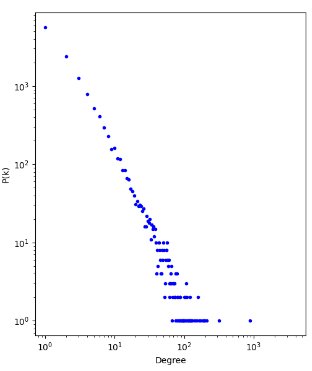
\includegraphics[width=0.8\linewidth]{img/degree_distribution.png}
  \caption{Degree distribution}
  \label{fig:Degree distribution}
\end{figure}

\noindent In Figure ~\ref{fig:Degree distribution}, the graph simply plots the degree values on the X axis and the number of nodes for each degree value on the Y axis.

\begin{figure}[hbpt]
  \centering
  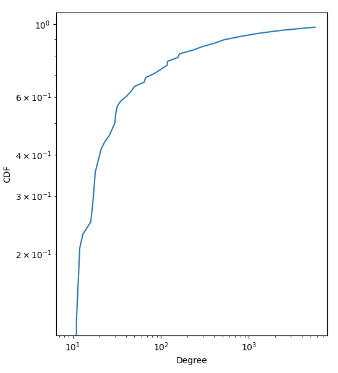
\includegraphics[width=0.8\linewidth]{img/degree_CDF.png}
  \caption{CDF (Cumulative Distribution Function)}
  \label{fig:CDF}
\end{figure}

\begin{figure}[hbpt]
  \centering
  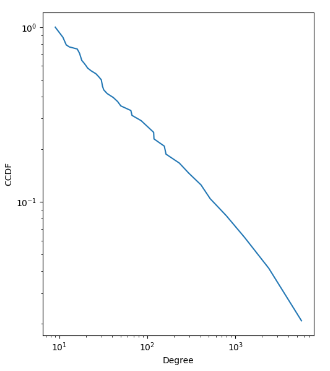
\includegraphics[width=0.8\linewidth]{img/degree_CCDF.png}
  \caption{CCDF (Complementary Cumulative Distribution Function)}
  \label{fig:CCDF}
\end{figure}

\noindent The graphs in Figure ~\ref{fig:CDF} and Figure ~\ref{fig:CCDF} represent respectively the Cumulative Distribution Function and the Tail distribution. The trend of both graphs shows that our network has an exponential distribution.

\subsubsection{Connected component analysis}  Before calculating the number of network components we wanted to try to represent the ego-network of the first node but the graph was not interesting.
Using the \textit{connected\_components()} method we calculated the number of components, which turned out to be 299. We then tried to identify a giant component, removing all nodes that were not part of it. The result is that we have gone from 299 to a single connected component and this component is made up of 12676 nodes. If the initial number of nodes was 13171, it means that the other 298 connected components were made up of 495 nodes, i.e. less than 4\% of the total number of nodes.

\subsubsection{Path analysis} The diameter measures 12 and the average shortest path corresponds to 4.31. We can notice that the average shortest path is 1/3 of the diameter.

\subsubsection{Global clustering coefficient and Density} The coefficient is equal to 0.045, which is a low value, meaning that the nodes on the graph have a low tendency to form closely related groups or clusters. Additionally, the density is 0.00042: it suggests the graph is relatively sparse, since the density indicates the fraction of connections actually present compared to the maximum number of connections possible. In this case there are few connections between nodes.

\subsubsection{Centrality analysis}  
Firstly, we investigated the number of interactions of each node by computing their degree centrality. The following table shows the top five nodes with the highest degree.
\begin{table}[htbp]
\centering
\caption{Degree Centrality}
\begin{adjustbox}{scale=0.85}
\begin{tabular}{lr}
\toprule
Username & Valore \\
\midrule
hi\_there\_bitch & 892 \\
TerrySharpHY & 321 \\
TwoCoresOneThread & 212 \\
perturbaitor & 199 \\
ClinicalIllusionist & 195 \\
\bottomrule
\end{tabular}
\end{adjustbox}
\end{table}

Then we analysed the centrality of the nodes in the network from different points of view using the following measures: closeness centrality, betweenness centrality, harmonic centrality, PageRank and EigenVector centrality.



\begin{figure}[!ht]
  \centering
  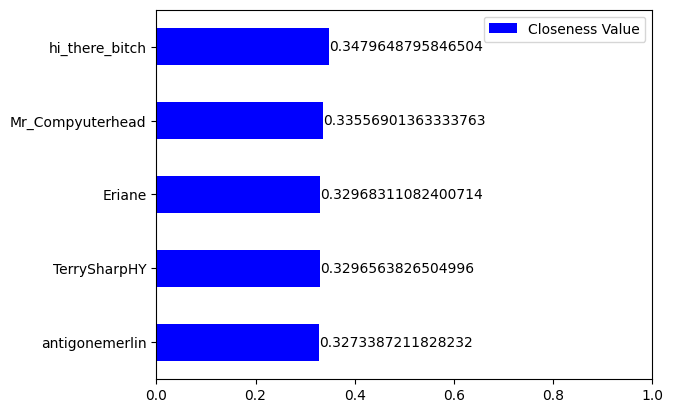
\includegraphics[width=0.4\textwidth]{closeness.png}
  \caption{Closeness Centrality}
  \label{fig:closeness_centrality}
\end{figure}

\begin{figure}[htbp]
  \centering
  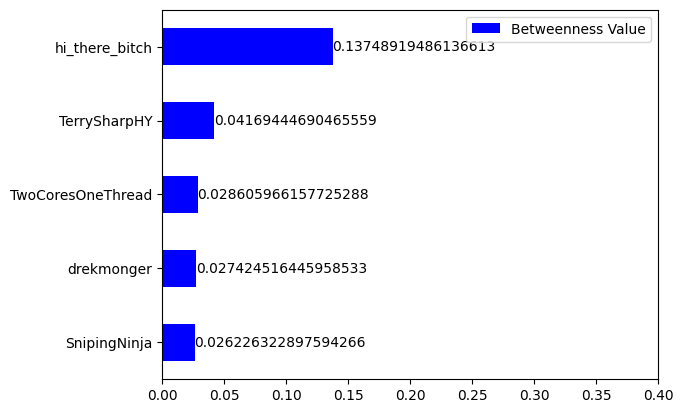
\includegraphics[width=0.4\textwidth]{betweenness.png}
  \caption{Betweenness Centrality}
  \label{fig:betwenness_centrality}
\end{figure}




Figures ~\ref{fig:closeness_centrality} and ~\ref{fig:betwenness_centrality} show the results of the closeness and the betweenness centrality analysis. 
Closeness centrality is a measure that quantifies how influential a node is in a graph and it enables us to evaluate how easily a node can reach other nodes in the graph; while betweenness centrality assesses the importance of a node based on its ability to act as an intermediary between other nodes.
By looking at the results shown in Figure ~\ref{fig:betwenness_centrality}, one could argue that there are no nodes that play a critical role in connecting different parts of the network. In fact, the betweenness centrality scores are very low, below 0.15. It can also indicate that the network is made of unconnected components.


\begin{table}[!htbp]
\centering
\caption{Other Centrality Measures}
\begin{adjustbox}{scale=0.5}
\begin{tabular}{ccc}
\toprule
\multicolumn{1}{c}{Eigenvector} & \multicolumn{1}{c}{PageRank} & \multicolumn{1}{c}{Harmonic} \\
\midrule
\begin{tabular}{lr}
Username & Value \\
\midrule
hi\_there\_bitch & 0.505 \\
TerrySharpHY & 0.116 \\
antigonemerlin & 0.108 \\
Mr\_Compyuterhead & 0.107 \\
perturbaitor & 0.101 \\
\bottomrule
\end{tabular} &
\begin{tabular}{lr}
Username & Value \\
\midrule
hi\_there\_bitch & 0.015 \\
TerrySharpHY & 0.005 \\
TwoCoresOneThread & 0.003 \\
ClinicalIllusionist & 0.002 \\
perturbaitor & 0.002 \\
\bottomrule
\end{tabular} &
\begin{tabular}{lr}
Username & Value \\
\midrule
hi\_there\_bitch & 5182.211 \\
Mr\_Compyuterhead & 4758.623 \\
TerrySharpHY & 4721.580 \\
Eriane & 4656.199 \\
antigonemerlin & 4636.908 \\
\bottomrule
\end{tabular} \\
\bottomrule
\end{tabular}
\end{adjustbox}
\end{table}

As we have seen so far, the users that play the most central roles are basically the same in every centrality analysis we conducted and they are also the ones with the highest number of connections.
Finally, we employed Newman’s Assortativity to quantify homophily, namely the tendency of nodes with similar characteristics to be connected to each other. The resulting assortativity coefficient is: -0.066. 
A negative assortativity coefficient indicates disassortative mixing, thus nodes tend to connect to others with different properties. For instance, high-degree nodes connect with low-degree nodes.

\subsection{Comparision with ER and BA graphs}
To build the Erdos-Renyi graph (ER) we needed the value of the probability of the edges creation. In order to find it, we used the following formula:

\[
p = \frac{2L}{N(N-1)} = \frac{240948}{13171 \cdot 13170} = 0.0004721262694
\]

Since the ER graph is constructed through the use of a probability, the number of edges resulting at each execution of the code varies, although they remain around the real value.
While for the construction of the Barabási-Albert graph we calculated the number of edges by the number of nodes multiplied by \textit{m}, which we obtained from the following formula:

\[
m = \frac{\langle k \rangle}{2} = \frac{6.217902968643231}{2} = 3.1089514843216155
\]

Thus, the ER graph has 40739 edges, while the BA graph has 39504 edges.

Comparing the results of the degree distribution with those of the real network we noticed that the average degree in the ER graph changes a little, approximately 6.18, compared to 6.21, while the number of connected components drops to 28, compared to the 299 of the real network. Even the graphs related to the degree distribution change a lot, they no longer represent an exponential distribution, but instead they show a normal one (Figure ~\ref{fig:degree_distribution_ER}, ~\ref{fig:CDF_ER} and ~\ref{fig:CCDF_ER}). The regime type of this graph is supercritical, as the value of p is greater than 1/N, which is 0.000076. The BA graph, on the other hand, is closer to the results of the real network, with the average degree being approximately 6 (5.99) and also the degree distribution graphs are similar to those of the real network. The number of connected components is 1, resulting in a single giant component.

\begin{figure}[hbpt]
  \centering
  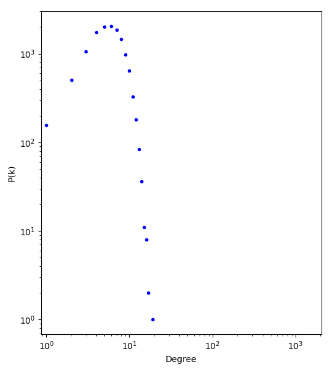
\includegraphics[width=0.8\linewidth]{img/degree_distribution_ER.png}
  \caption{Degree distribution of ER graph}
  \label{fig:degree_distribution_ER}
\end{figure}

\begin{figure}[hbpt]
  \centering
  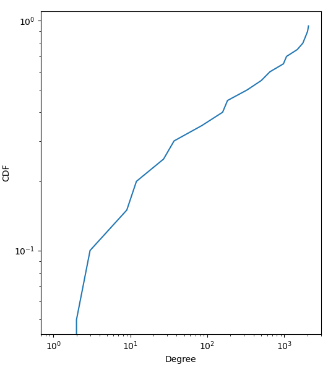
\includegraphics[width=0.8\linewidth]{img/CDF_ER.png}
  \caption{CDF of ER graph}
  \label{fig:CDF_ER}
\end{figure}

\begin{figure}[hbpt]
  \centering
  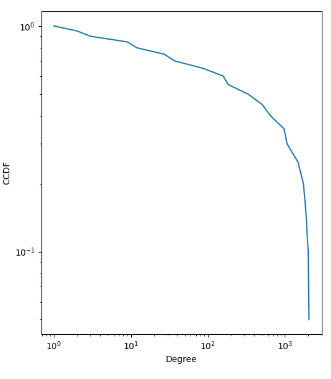
\includegraphics[width=0.8\linewidth]{img/CCDF_ER.png}
  \caption{CCDF of ER graph}
  \label{fig:CCDF_ER}
\end{figure}

With regard to the centrality analysis, for both Erdos-Renyi and Barabási-Albert graph we have chosen to display the top five results of the following centrality measures: Degree, Closeness and Betweenness centrality (Table ~\ref{fig:centrality_measures_ER_BA}). Nevertheless, the Degree Centrality results appear to be the most relevant. 

\begin{table}[h]
\centering
\caption{Centrality Measures in ER and BA graphs}
\adjustbox{width=0.5\textwidth}{
\begin{tabular}{ccccccc}
\hline
\label{fig:centrality_measures_ER_BA} \\
\multicolumn{3}{c}{ER GRAPH} & \multicolumn{3}{c}{BA GRAPH} \\
\hline
Degree C. & Closeness C. & Betweenness C. & Degree C. & Closeness C. & Betweenness C.\\
\hline
21 & 0.214 & 0.002 & 351 & 0.35 & 0.098 \\
18 & 0.213 & 0.002 & 291 & 0.35 & 0.083 \\
18 & 0.21 & 0.002 & 287 & 0.34 & 0.069 \\
17 & 0.21 & 0.001 & 228 & 0.34 & 0.062 \\
17 & 0.21 & 0.001 & 180 & 0.34 & 0.047 \\
\hline
\end{tabular}
}
\end{table}

In terms of nodes degree, the difference between the random network predictions and the real world network is attributable to the Poisson distribution, which minimizes the possibility of a node to have a high degree. In fact, according to the ER model the maximum degree should be 21.

\section{Network Manipulation and Analysis}

\subsection{Community detection}
This analysis focuses on discovering the network's structure, comparing and evaluating the results of the identified communities. 
Concerning crisp communities, the algorithms used are Louvain and Leiden.
Louvain algorithm has two phases repeated iteratively. Each node begins in its own community, then moves to the adjacent community that offers the biggest modularity boost. The graph is updated with communities connected by weighted links and bridges.
Leiden algorithm works as a hierarchical clustering that merges communities into single nodes. 

As far as overlapping communities are concerned, namely a node can belong to multiple communities, two algorithms are implemented: Demon and k-clique. Demon algorithm starts from the ego-networks, built upon a focal node. 
The ego node n is extracted and removed from the network, then label propagation is performed and n is placed in every identified community. Finally, if some communities are similar they are merged. 
Instead, a k-clique community is the union of all k-size clicks that can be achieved by adjacent k-cliques (sharing k-1 nodes).

Community-based evaluation is implemented through two strategies: internal evaluation and external evaluation.\vspace{8pt}

\vspace{5pt}
{\fontsize{10}{10}\selectfont \textit{Internal Evaluation }}

\begin{itemize}
  \item [-]\textbf{Conductance}: the fraction of total edge volume that points outside the community. \newline
\begin{center}
$f(S) = \displaystyle\frac{cS}{2mS + cS}$
\end{center}
 
\vspace{5pt}
\begin{flushleft}
In the formula \textit{cs} stands for number of community nodes and \textit{ms} represents the number of community edges
 \end{flushleft}
\vspace{10pt}
\end{itemize}

\begin{itemize}
\item [-]\textbf{Internal edge density}: the proportion of arcs connecting nodes within a specific community to the total number of possible arcs within that community
\vspace{4pt}

\begin{center}

$f(S) = \displaystyle\frac{mS}{\frac{nS(nS-1)}{2}}$
\end{center}

\vspace{5pt}
\begin{flushleft}
where \textit{mS} is the number of community internal edges and \textit{nS} is the number of community nodes.
 \end{flushleft}
  \end{itemize}

\vspace{10pt}

{\fontsize{10}{10}\selectfont \textit{External Evaluation }}
 

\begin{itemize}
  \item [-]\textbf{Overlapping Normalized Mutual Information} between two clusterings.

\vspace{5pt}
\item [-]\textbf{F1 score}: matches among the partitions
\end{itemize}


\begin{table}[htbp]
\centering
\caption{Community detection}
\adjustbox{scale=0.8}{
\begin{tabular}{cccccr}
\toprule
 & Parameter(s) & \#Community & Conductance & Altro \\
\midrule
Louvain & Resolution:2 &392 & 0.126 &  \\
Leiden & None & 335 & 0.046 \\
Demon & $\epsilon$:0.25 &110 &0.85\\
Angel & threshold:0.25 &1 &0.019\\
\bottomrule
\end{tabular}
}
\end{table}

[DA AGGIUNGERE]GRAFICI FINALI E COMMENTI 


\FloatBarrier

\subsection{Spreading}
Diffusive phenomena are analyzed using the \textit{ndlib} \cite{Rossetti_2017} library by considering the three stochastic epidemic models: SI, SIS, and SIR. 
In the first one the individuals can be in one of these two states: susceptible (S) or infected(i).  

In SIS model susceptible individuals become infected and each has a probability to revert its status to susceptible; whereas SIR susceptible individuals got infected but each one has a probability of becoming immune. 
These models applied to the network show symmetric pattern, so when a node becomes infected, its connectivity with other nodes might allow a high probability of transmission, causing an increase in infected nodes. Later, when the number of infected nodes reaches its peak, the effect of healing or control measures could cause a decrease in the number of infected nodes, leading to a symmetrical trend in the graph.
Although this distribution can be almost identical for every network, there may be differences in values due to system characteristics. Significance can be gained from analyzing the SIS and SIR models utilized, and some remarks can be made. The first one (Figure ~\ref{fig:immagine_sis}) has 6 peaks at different iterations with the delta value (3, -3). The SIR model (Figure ~\ref{fig:immagine_sir}) only has one peak approximately at the 160\textsuperscript{th} iteration with a delta value between 6 and -6.

\begin{figure}[H]
  \centering
  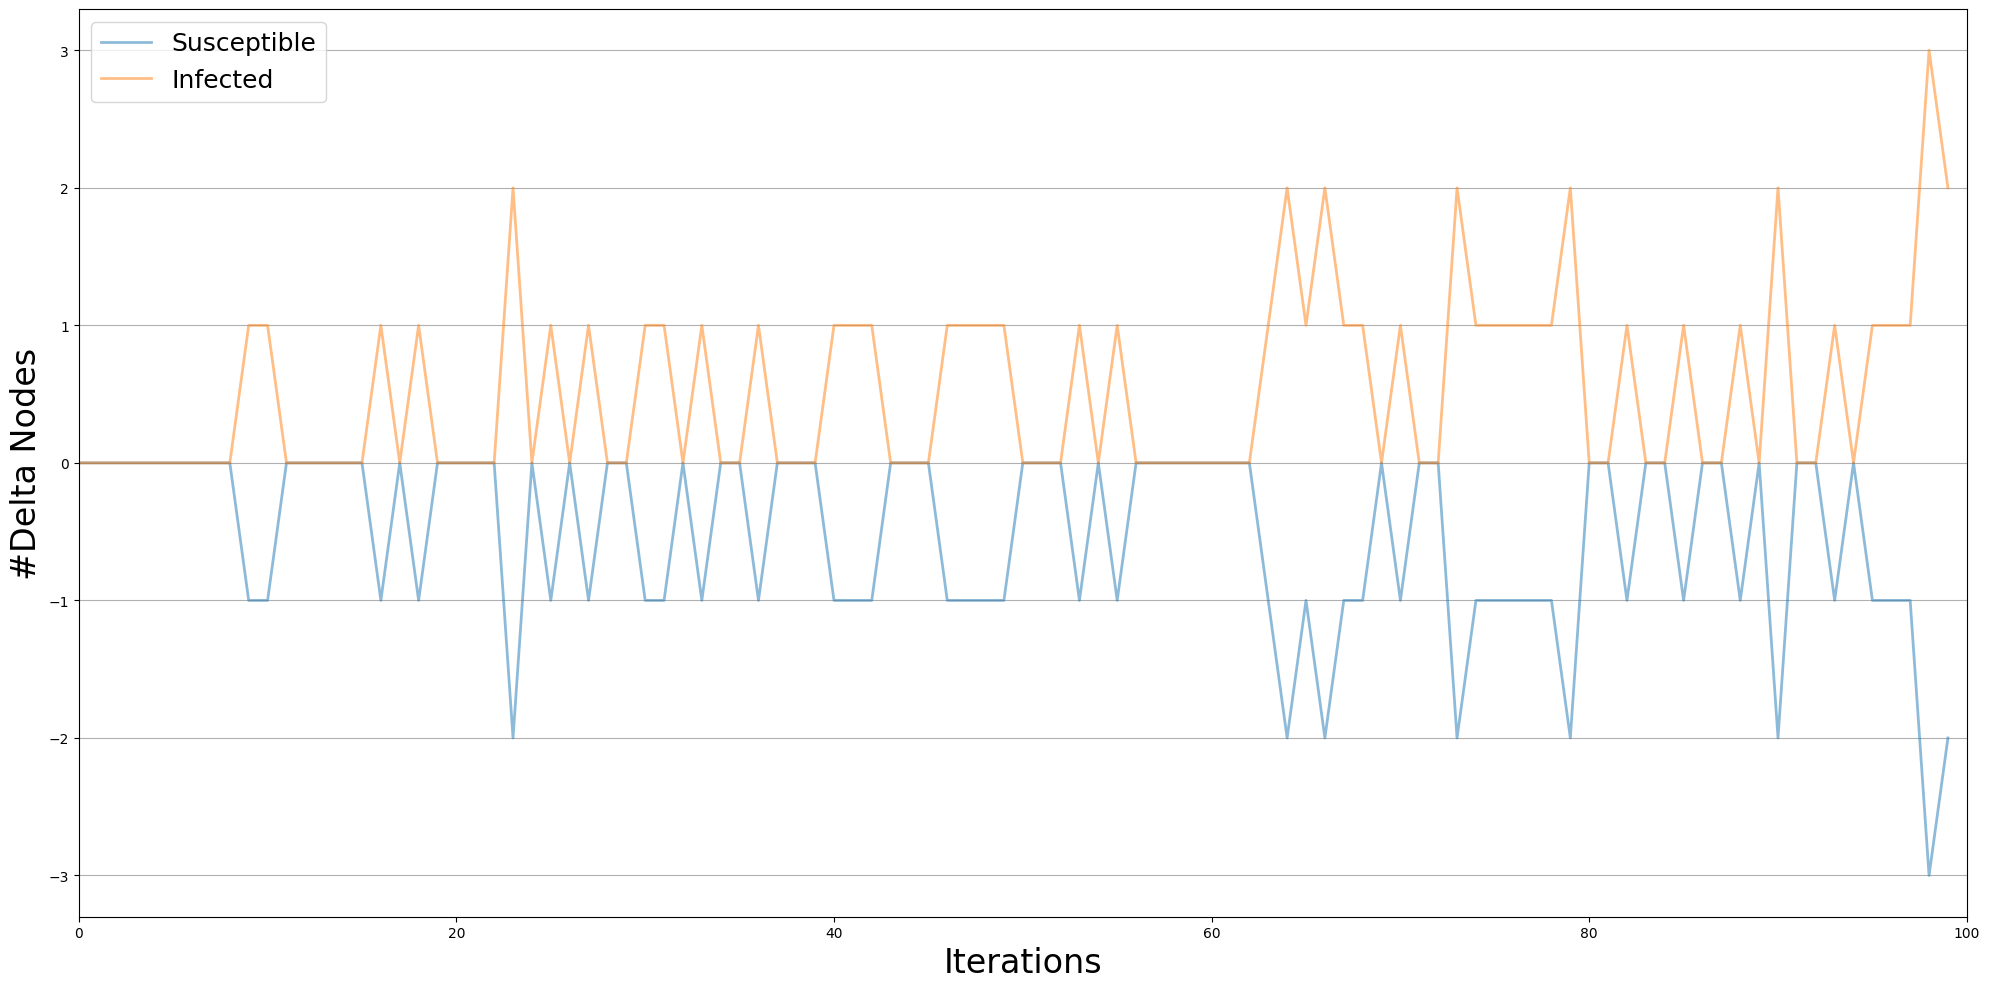
\includegraphics[width=0.50\textwidth]{si.png}
  \caption{SI model}
  \label{fig:immagine}
\end{figure}
\begin{figure}[H]
  \centering
  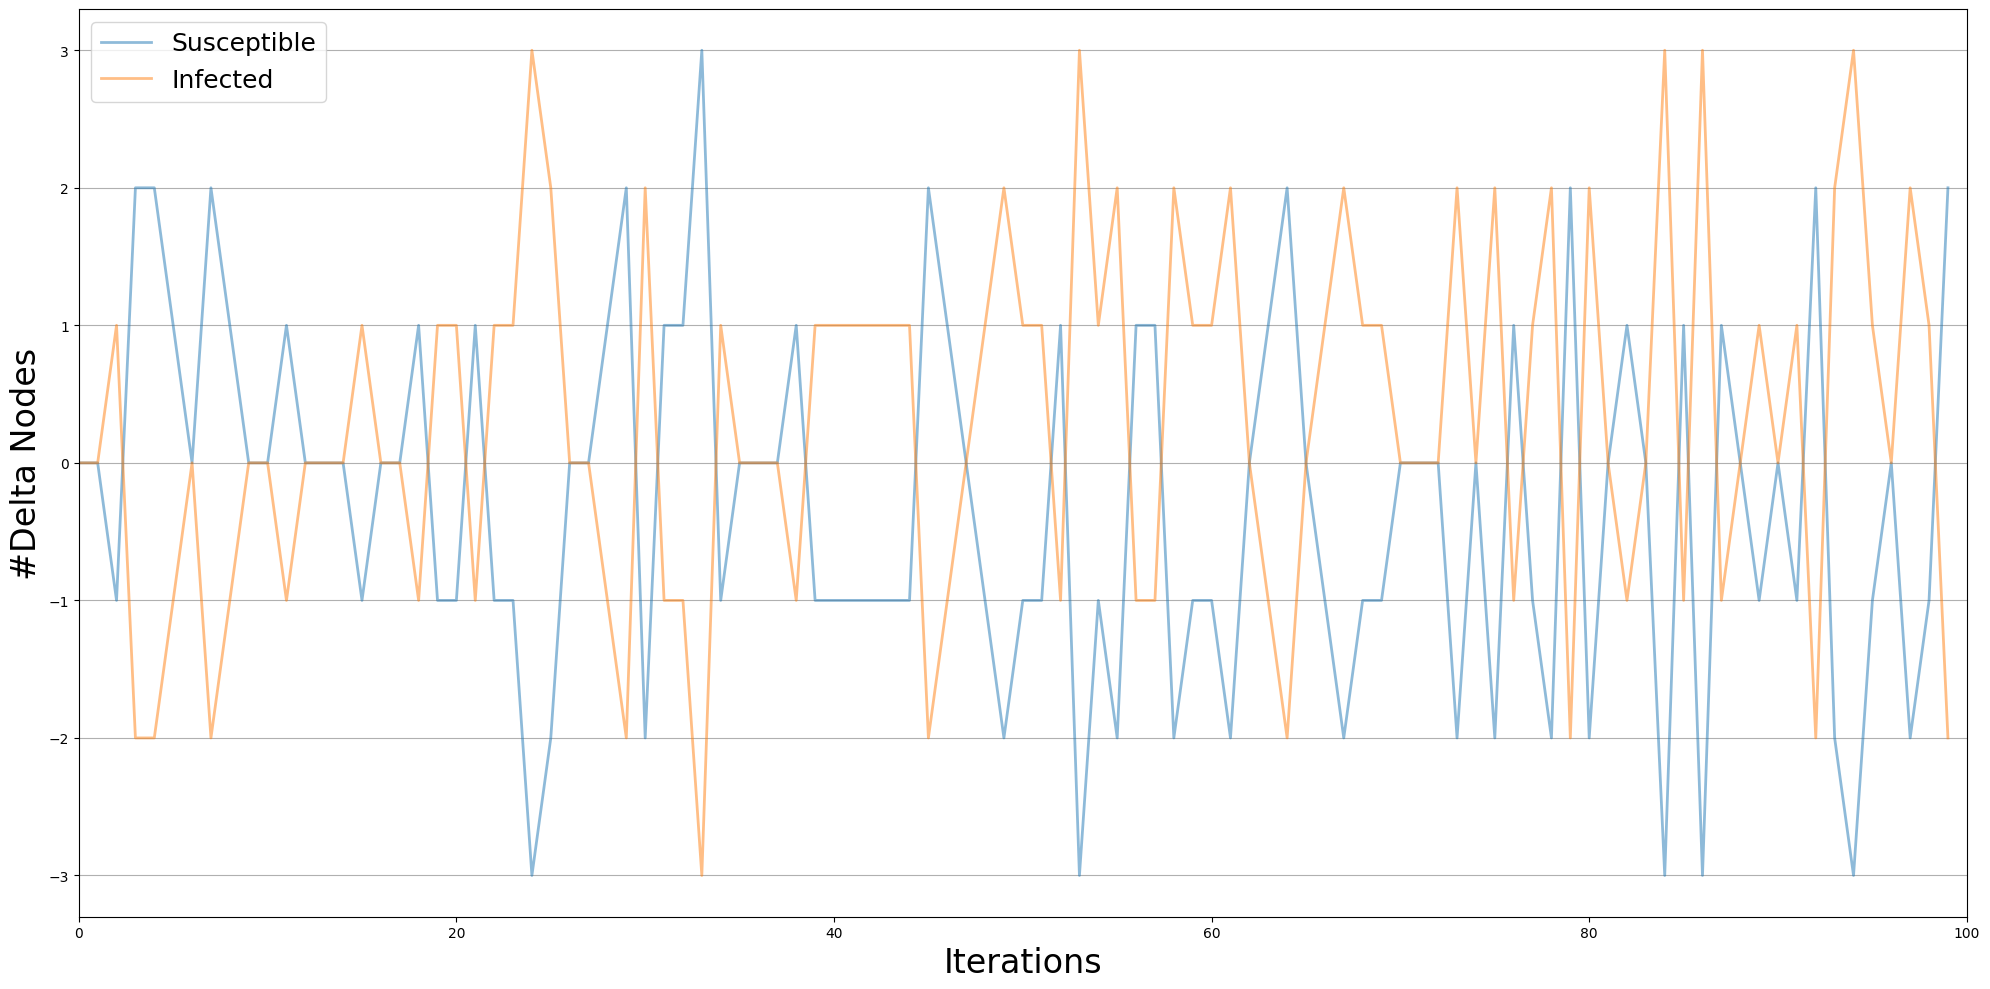
\includegraphics[width=0.50\textwidth]{sis.png}
  \caption{SIS model}
  \label{fig:immagine_sis}
\end{figure}

\begin{figure}[H]
  \centering
  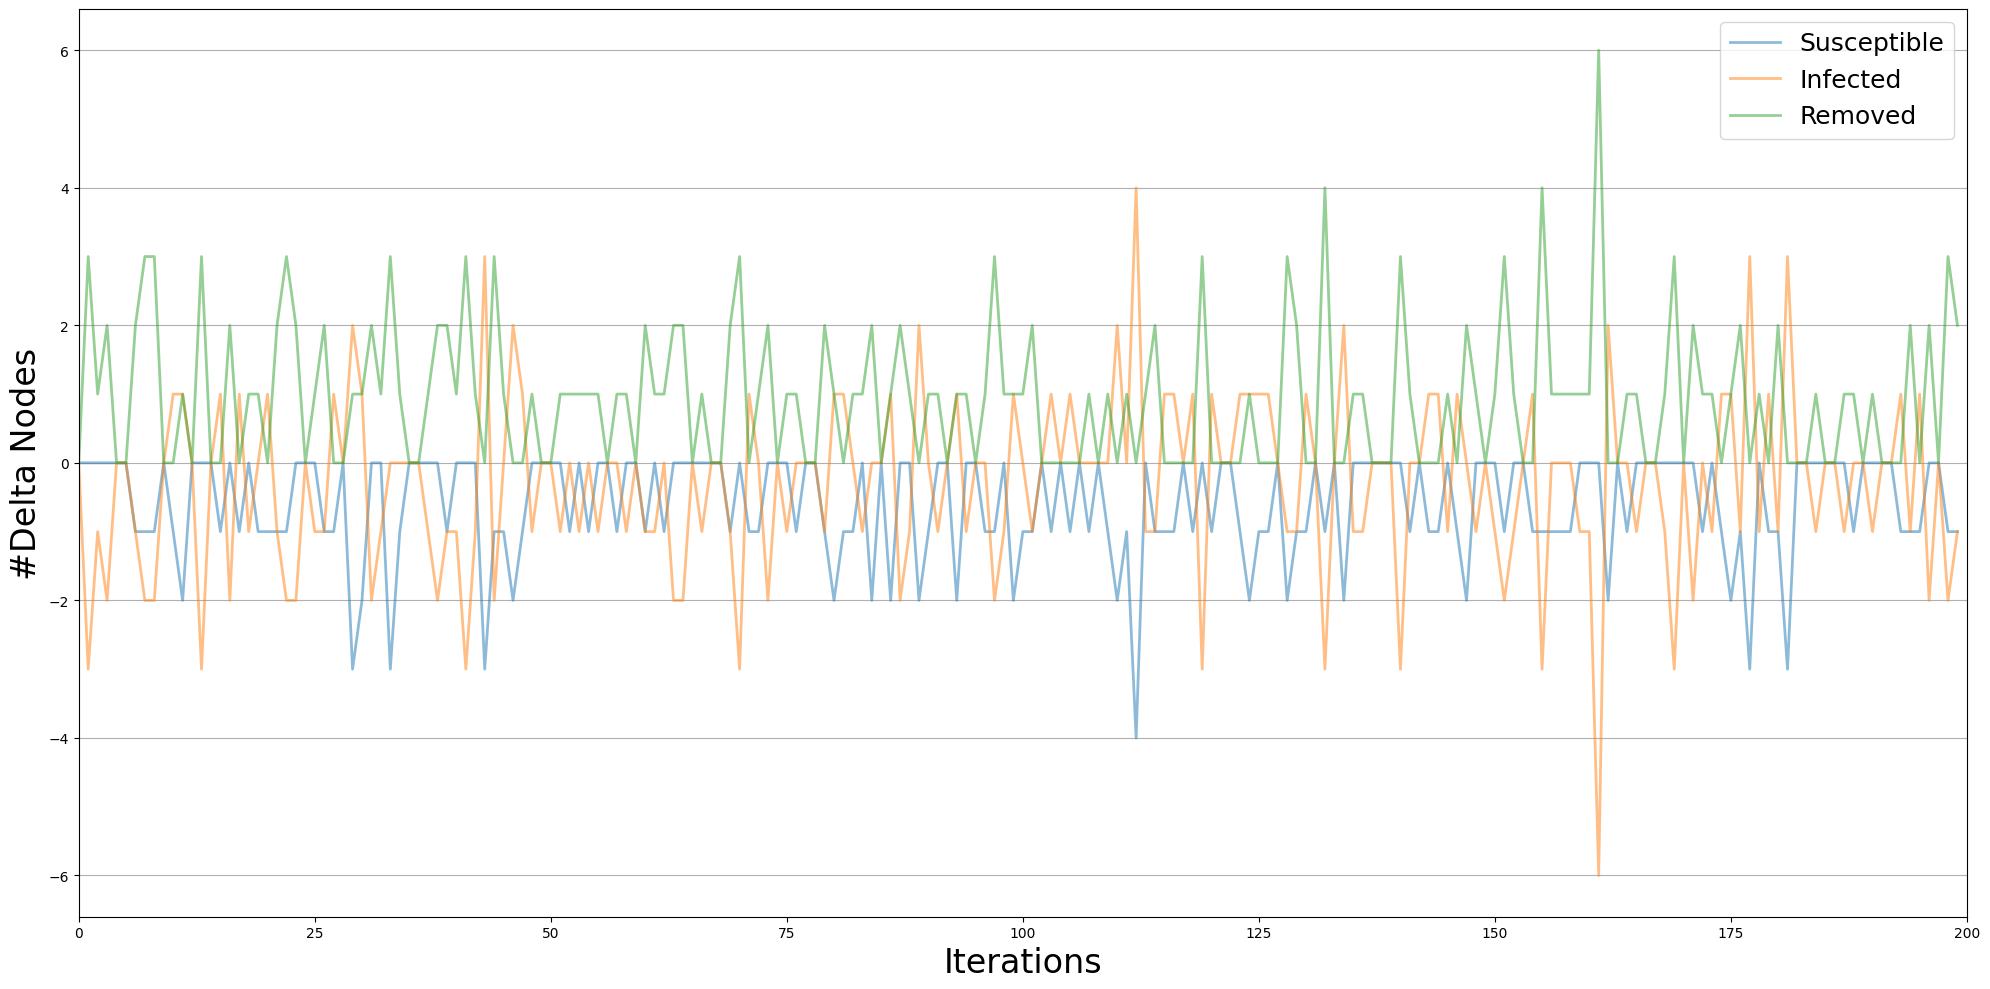
\includegraphics[width=0.50\textwidth]{SIR.png}
  \caption{SIR model}
  \label{fig:immagine_sir}
\end{figure}


\subsection{Higher-order Network Analysis}

Formally, a hypergraph is defined as a pair H = (V, E), where V is a set of nodes and E is a set of hyperedges. Each hyperedge in E can contain any number of nodes. To build the Hypergraph we used the library \textit{HyperNetX}\cite{doecode_22160}. We adapted our dataset to the format the library requested: we created a new attribute that specifies the edges between two nodes through a label. The resulting number of hyperedges is 49885. Then we investigated the cardinality of the hyperedges, which is the number of nodes contained in a hyperedge. 

\begin{table}[htbp]
\centering
\caption{Hyperedge Information}
\begin{tabular}{ccr}
\toprule
Cardinality & Number of Hyperedges \\
\midrule
2 & 48096 \\
1 & 1789 \\
\bottomrule
\end{tabular}
\end{table}


Hyperedges with two nodes are equivalent to traditional edges in a graph. The fact that the majority of hyperedges have a cardinality of 2 implies that the hypergraph focuses on pairwise connections; this also suggests the absence of higher-order relationships and complex interactions between larger sets of nodes. 
The hyperedges with cardinality equal to 1 represent a single node connected to itself: it could indicate the presence of self loops or isolated nodes. A visual representation of the hyperedges is portrayed in Figure\ref{fig:hypegrafi1}, in which hyperedges of both cardinality 1 and 2 are rendered.

\begin{figure}[htbp]
  \centering
  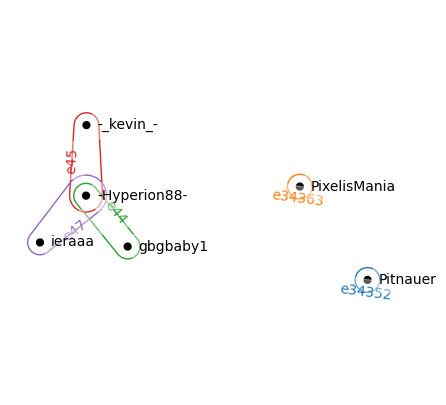
\includegraphics[width=0.4\textwidth]{hyperedges.png}
  \caption{Hyperedges.}
  \label{fig:hypegrafi1}
\end{figure}


This situation clearly represents the direct interactions between pairs of users in the network.  \\
Additionaly, we devided the number of hyperedges by the number of nodes to obtain the connectivity measure. The result was 3.79. \\
Finally, we investigated the modularity of the hypergraph to measure the quality of its partions. 
Before applying the modularity algorithm we used Kumar clustering algorithm, which is a method that uses the Louvain algorithm to create a partition of the vertices. The resulting modularity score is 0.51. The modularity score ranges from -1 to 1, with higher values indicating a stronger community structure. Thus, this modularity score suggests a moderate level of community structure in the network.



\subsection{Dynamic Network Analysis}
The Dynamic Network Analysis was done using \textit{DyNetX}\cite{DynetX}, a Python library that extends networkx for dynamic network modelling. 

\noindent We modelled our data by creating several 'Network Snapshots', then generating Snapshot Graphs to represent, as a dynamic phenomenon to be observed, the evolution of our graph over certain time intervals.

\noindent In the phase preceding the construction of the Dynamic Network, of which the Snapshots Graph is composed, the time interval was discussed. 

\subsubsection{Data pre-processing / DynGraph settings} 
The dataset on which our analysis is based contains data from December 2022, 
therefore the creation of the Dynamic Network focused on a 4-week time interval, observing its evolution with each addition of the arcs according to their intuitively increasing periods of appearance. 

The total dates on which we investigate are 30, from 02/12/22 to 30/12/22 inclusive.
Having imported a time window of 7 days, the total number of groups/classes indicating them, (i.e. interactions/edges) is 4. Therefore, each row of the dataset has been labelled by adding a \textit{Time t} column according to the corresponding date, in ascending date order.

The Dynamic Graph is then constructed by adding the edges from the dataset in order of time of appearance, so from time 0 to time 4, while the nodes of the network exist from time 0, resulting with 13170 nodes and 33741 edges.

\subsubsection{Snapshots Analysis} From the Dynamic Graph we can access to each different temporal snapshot, whose data are reported in the following Table \ref{tab:Snapshots Nodes and Edges}.


\begin{table}[htbp]
\centering
\caption{Snapshot's Nodes and Edges}
\label{tab:Snapshots Nodes and Edges}
\begin{tabular}{|c|c|c|}
\hline
\centering
    Snapshot & Number of Nodes & Number of Edges \\
    \hline
    0 & 1798 & 3186 \\
    1 & 6250 & 13449 \\
    2 & 9838 & 23317 \\
    3 & 13170 & 33741 \\
\hline
\end{tabular}
\end{table}

\vspace{1pt} % Spazio verticale tra la tabella e il testo
From the number of nodes and edges, we can see that as the time intervals grow, and therefore as edges are added to the network, we can say, as we anticipated earlier, that the network grows. In fact, we note that in the last snapshot, where we have the complete graph showing the data for the entire month, it includes all nodes and edges.


\noindent Similarly, it is possible to obtain snapshots of longer time intervals, e.g. we can obtain data from a Snapshot ranging from time t=0 to t=2 and see the state of the graph in that time span:

\vspace{5pt}

\noindent \texttt{Number of nodes in the interval: 9838}

\noindent \texttt{Number of edges in the interval: 23317}

\noindent \texttt{Interaction per Snapshot {0: 1631.0, 1: 6855.5}}

\vspace{5pt}

We note that nodes and edges correspond precisely to those in Snapshot 2 in the Table \ref{tab:Snapshots Nodes and Edges} above. While for the interactions, the 0 key indicates interactions observed in the first week of the month, instead the 1 key indicates interactions observed from the first to the second week, i.e. it counts whether the arcs starting from the observed week remain present until the end of the time interval.


\noindent \subsubsection{Dynamic Network Measures} Finally, in the next tables we can observe the measurements performed on the constructed Dynamic Graph, some of which refer to two generic nodes u and v, chosen randomly.

\noindent The first measures, reported in Table \ref{tab:Inter Event Time Measures}, regard the Inter Event Time Measure (IET), that indicates how much time occurs before a new interaction appears in the graph. 

\begin{table}[!ht]
\centering
\caption{Inter Event Time Measures }
\label{tab:Inter Event Time Measures}
\begin{tabular}{|c|c|}
\hline
\textbf{IET} & \textbf{N. Interactions} \\ \hline
\textbf{Global} & \begin{tabular}[c]{@{}c@{}}temporal distance\\ \{0: 34728, 1: 3\}\end{tabular} \\ \hline
\textbf{Node} & \begin{tabular}[c]{@{}c@{}}temporal distance\\ \{0: 2, 2: 1\}\end{tabular} \\ \hline
\textbf{Edge} & \begin{tabular}[c]{@{}c@{}}temporal distance \\ \{3: 1\}\end{tabular} \\ \hline
\end{tabular}
\end{table}

We can notice that in the value of Global measurement, therefore taking into account the whole month, just in one of the four snapshots there are three new interactions.

In the Table \ref{tab:Dynamic Network Measures} below, instead, are reported the measure of: \textit{Coverage} (C) that is the ratio of existing nodes w.r.t. the possible ones; \textit{Coverage of Node/Edge} (CNE) which reports the coverage of w.r.t. a node 'u' and of edge (u, v), \textit{Pair Uniformity} (PU) that is the overlap between the presence times of u and v; \textit{Density} (D) that indicates the temporal network density, which is the fraction of possible interactions that do exist in the temporal network and \textit{Node Density}, (ND) \textit{Pair Density} (PD) which respectively indicate the intersection between the node/edge's temporal presence and the joint node/edge's temporal presences.

\vspace{10pt}

\begin{table}[htbp]
\centering
\begin{tabular}{|c|c|}
\hline
\textbf{Measure} & \textbf{Value} \\ \hline
C & 0.59 \\ \hline
CNE & \{Node: 1.0, Edge: 1.0\} \\ \hline
PU & 1.0 \\ \hline
D & 0.0004634 \\ \hline
ND & 0.0004507 \\ \hline
PD & 1.0 \\ \hline
\end{tabular}
\caption{Dynamic Network Measures}
\label{tab:Dynamic Network Measures}
\end{table}


The \textit{Snapshot Density} measure, on the other hand, shows us that the Snapshot Networks taken individually all give very low values, with the densest being the one at snapshot one with a value of 0.0020, consistent with the observed density of a single node w.r.t. the entire graph in Table \ref{tab:Dynamic Network Measures}; as the network grows it decreases more and more, emphasising the increase in edges but the sparsity of inspected network.

\subsubsection{Study of stability} The stability study was done to observe changes over time between snapshots by questioning four metrics: Jaccard Coefficient, Clustering Coefficient, Degree Centrality and a comparison of the Degree Distribution.
\\

\noindent The \textit{Jaccard Coefficient}: the highest value was recorded between Snapshots at time t=2 and t=3 with 0.67 which tells us that there were few changes in that timeframe, i.e. there was a low addition to the exchange of responses; whereas the lowest value was recorded between Snapshots at time t=0 and t=1 with 0.22, which tells us that there were few nodes that interacted with each other between the first and second week.
\\

\noindent The \textit{Clustering Coefficient}: The highest value was recorded in the Snapshot at time t=0 with 0.057 which tends to decrease slightly until the last Snapshot at time t=3 with 0.043.
They both remain very small values, which indicate that the tendency of a node's neighbours to be connected to each other is very low from the start, and as the network grows this tends to decrease.
\\

\noindent The \textit{Degree Centrality}: as the results we obtained show, the node that has the highest degree centrality in every snapshot is \textit{'hi\_there\_bitch'}, which has the value of 0.11 at time t = 2. Despite this fact, the values of degree centrality of all nodes prove that the network is sparse at all times.

\begin{figure}[!ht]
  \centering
  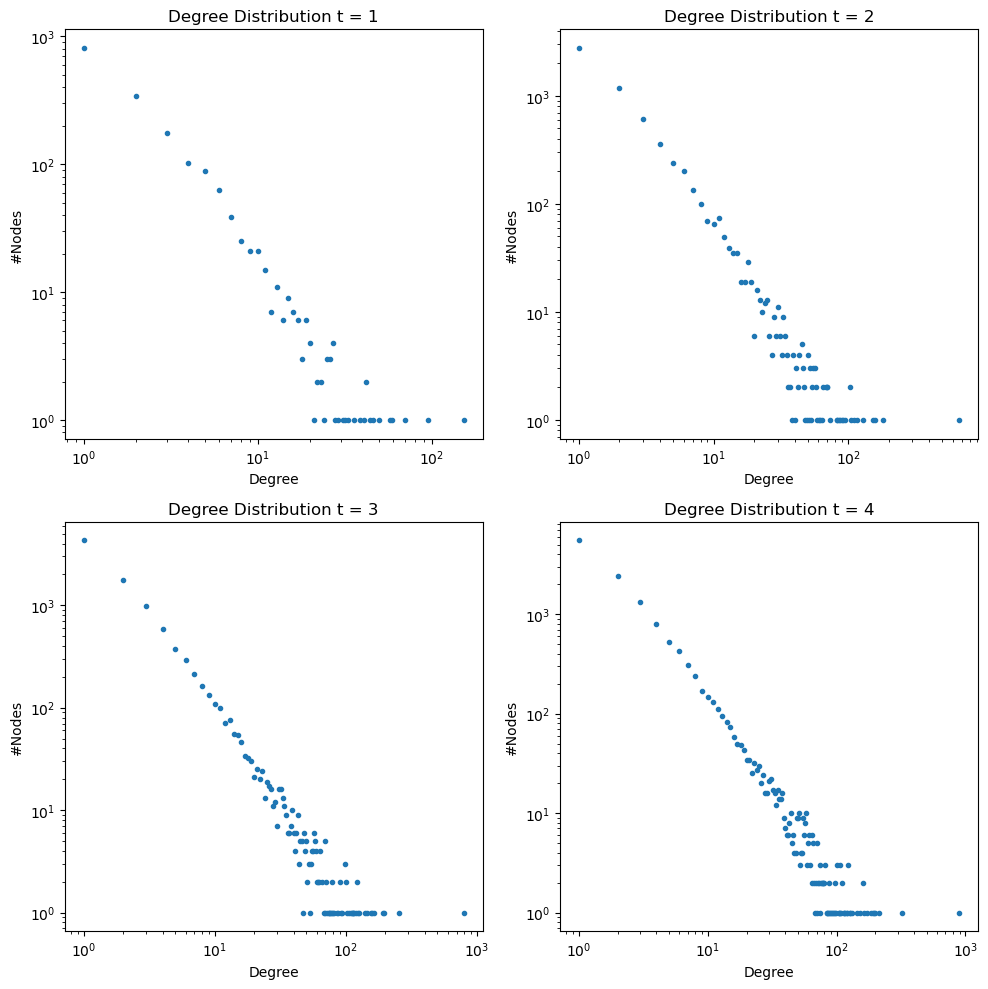
\includegraphics[width=0.4\textwidth]{img/dd_snapshot.png}
  \caption{Degree Distribution of each Snapshot}
  \label{fig:Degree Distribution Snapshot}
\end{figure}


In conclusion, as we can see in the Figure \ref{fig:Degree Distribution Snapshot} there are few changes in density, taking into account a total time window of one month, indicating again that the network is evolving over time, growing slowly.

\section{open questions}
In this section we investigate which are the main subject areas the comments fall into. The research question we asked ourselves was: \textit{`In which topics is chatGPT most used/discussed by users?'}. In order to determine that, we carried out a topic modeling analysis. We used a transformer-based model named BERTopic, which is an open-source library that uses a BERT model to do Topic Detection with an TF-IDF (Term Frequency - Inverse Document Frequency) algorithm that weights the importance of words in a corpus. The importance depends on the word's frequency: the more frequent a word is, the more important it is. The aim of the analysis is to get an overview of the main topics of the comments we retrieved.\\

We prepared the data with a pre-processing that included the removal of the stop words, since their high frequency can cheat the extraction. We also looked for capital letters and special characters. After this verification, the list of the comments was submitted to the model. 
Only a small representative portion of 1300 comments was given. \\ The topics extracted were visualized through different kinds of graphs. The most relevant is the barchart (Figure ~\ref{fig:immagine_bar}) and it shows the main topics identified and for each one it displays the internal subjects covered. 



\begin{figure}[H]
  \centering
  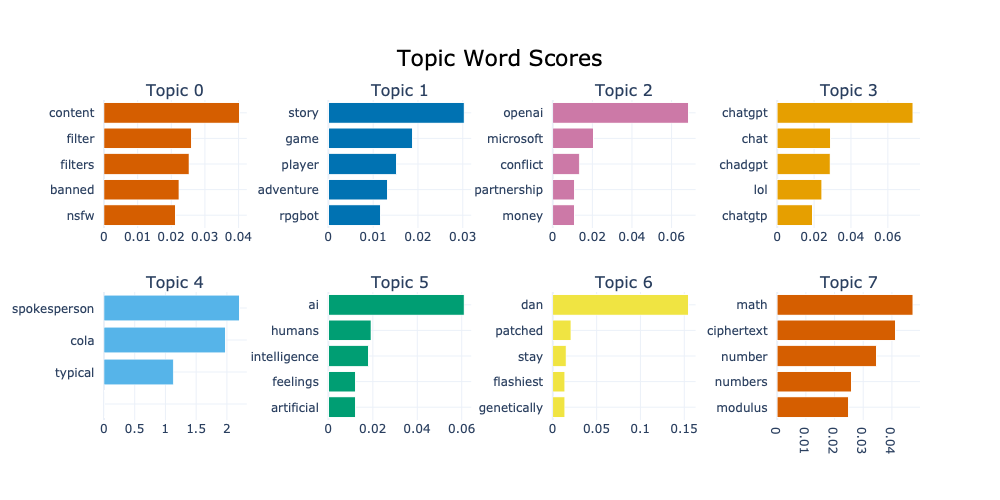
\includegraphics[height=5cm]{barchart.png}
  \caption{Barchart of the Topic Word Scores}
  \label{fig:immagine_bar}
\end{figure}



Finally, the test part is performed through the use of different probability measures that reveal to which extent the sentences belong to the topic identified. There are three parameters:
\begin{itemize}
  \item \textbf{Topic}: which contains the id of the topic
  \item \textbf{Count}: that refers to the number of the sentences belonging to a particular topic
  \item \textbf{Name}: the automatically generated topic label. 
\end{itemize}The top `-1' topic is assumed as irrelevant.  

The analysis provided eight different topics. We found the most relevant to be: \textit{history, games, Microsoft} and \textit{mathematics}.

After the recognition of the main topics, other specific analyses are carried out, namely sentiment analysis and the detection of the dominant matter in each topic. 



\subsection{Insight into the topics}
After the topic identification by Bert, an in-depth study about them is developed to understand more specifically what people could ask to chatGPT in relation to the different arguments identified. The analysis starts from the Named-Entity Recognition (NER), a method that extracts information from the given text. It consists of identifying the named entities referring to the key topics of the text, in this case comments, such as names, locations, companies, products, events. First, the comments about that topic are extracted by using topic keywords such as \textit{history}, \textit{game}, \textit{Microsoft}, \textit{math}. The NER process is accomplished by considering only \textsc{PER}, which is the name of people, and \textsc{ORG}, which is the name of different types of organizations. Frequency of words is achieved by obtaining key words that can inform about the most commonly discussed topic among people. Lastly, a graphic linking the keywords, represented by nodes, is constructed. The number of words is not a fixed number, as everything is dependent on the topic. 
 

\begin{figure}[H]
  \centering
  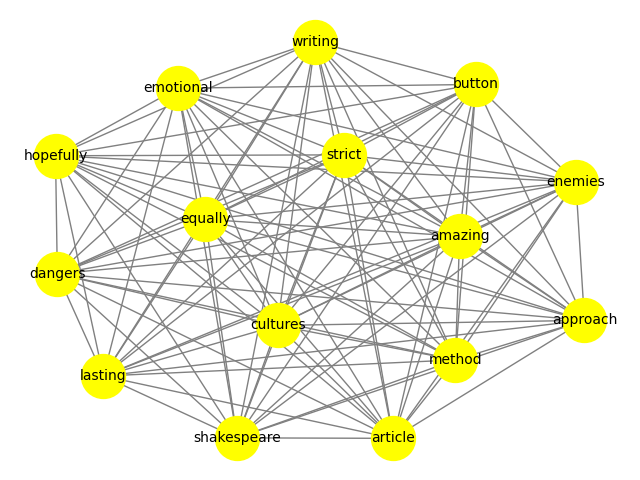
\includegraphics[width=0.4\textwidth]{primo.png}
  \caption{Graph for history topic}
  \label{fig:immagine_history}
\end{figure}



\begin{figure}[H]
  \centering
  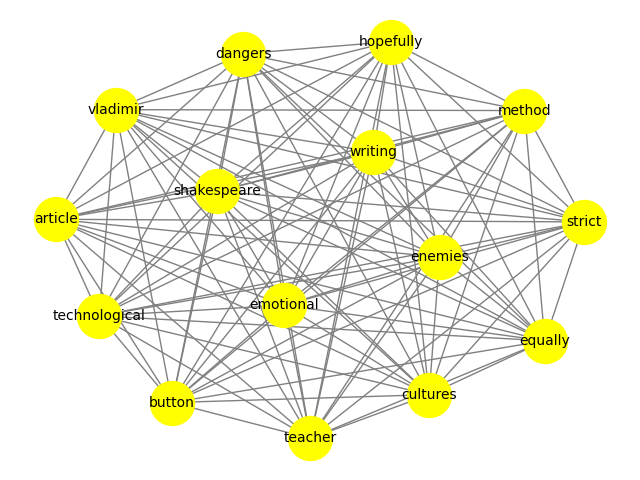
\includegraphics[width=0.4\textwidth]{secondo.png}
  \caption{Graph for game topic}
  \label{fig:immagine_game}
\end{figure}


\begin{figure}[H]
  \centering
  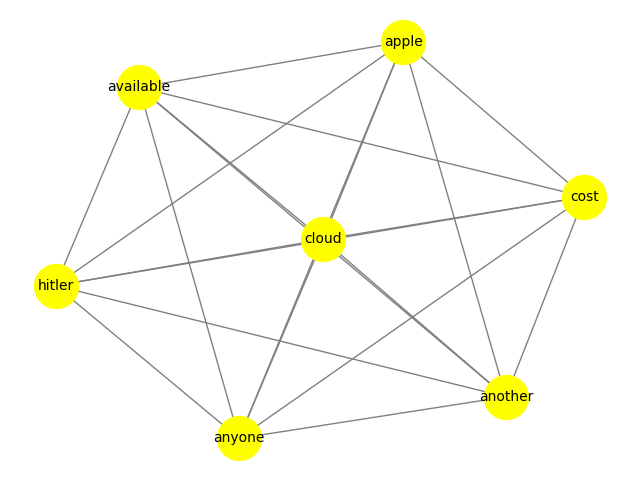
\includegraphics[width=0.4\textwidth]{terzo.png}
  \caption{Graph for Microsoft topic}
  \label{fig:immagine_mi}
\end{figure}

\begin{figure}[H]
  \centering
  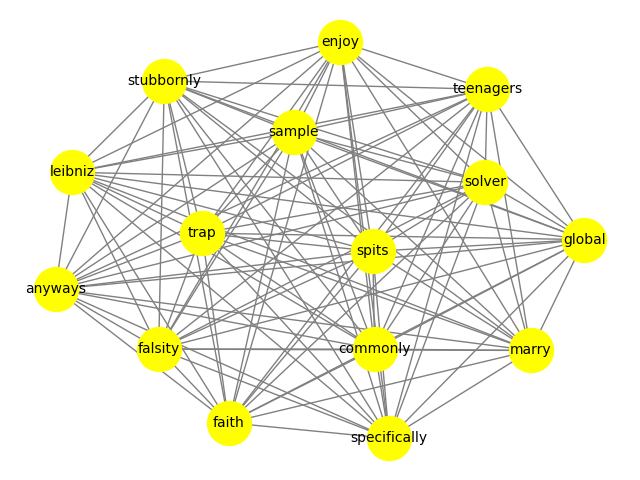
\includegraphics[width=0.4\textwidth]{quarto.png}
  \caption{Graph for math topic}
  \label{fig:immagine_math}
\end{figure}

In the following results what emerges are words related to topics. The first graph ~(Figure \ref{fig:immagine_history}) about history contains terms such as \textit{Shakespeare}, \textit{enemies}, \textit{method}, \textit{writing}, \textit{cultures}. It could be possible that people asked ChatGPT to help them with a task, for instance writing an article or looking for one.

In the second one ~(Figure \ref{fig:immagine_game}), that concerns the gaming area, there are several common words such as \textit{dangers}, \textit{method}, \textit{technological}, \textit{enemies}. Probably the users talk about these games to ChatGPT to find some strategies or just to take some information. 

The third graph ~(Figure \ref{fig:immagine_mi}) is regarded to Microsoft, so what is expected is to find some technological terms, indeed there are words as \textit{cloud}, \textit{avalaible}, \textit{apple}, but what is stranger is to find term like \textit{hitler}, that should belong to the history topic. In the math topic graph ~(Figure \ref{fig:immagine_math}) there are few words connected to the argument as \textit{Leibniz}, \textit{solver}, \textit{sample}, \textit{specifically}, but the majority of the words are not relevant.

\subsubsection{Sentiment analysis} Through this analysis the general idea of the users' opinion about ChatGPT can be inferred. The library used is TextBlob, which is a Python library for natural language processing (NLP) that simplifies information extraction from text and offers features such as sentiment analysis, sentence extraction, tokenization, lemmatization, part-of-speech classification, and more. As first step the stop words are removed to avoid having particular influences in the analysis. For each sentence is computed the \textit{sentiment} which is delivered as a score; in relation to it the sentence can be classified as Positive (score greater than 0), Negative (score less than 0), of Neutral(other score values). The visual distribution is realized by a bar chart (Figure ~\ref{fig:immagine_sentiment}) , which discloses that the majority of the opinions about Chat GPT are rated as positive. 

\begin{figure}[H]
  \centering
  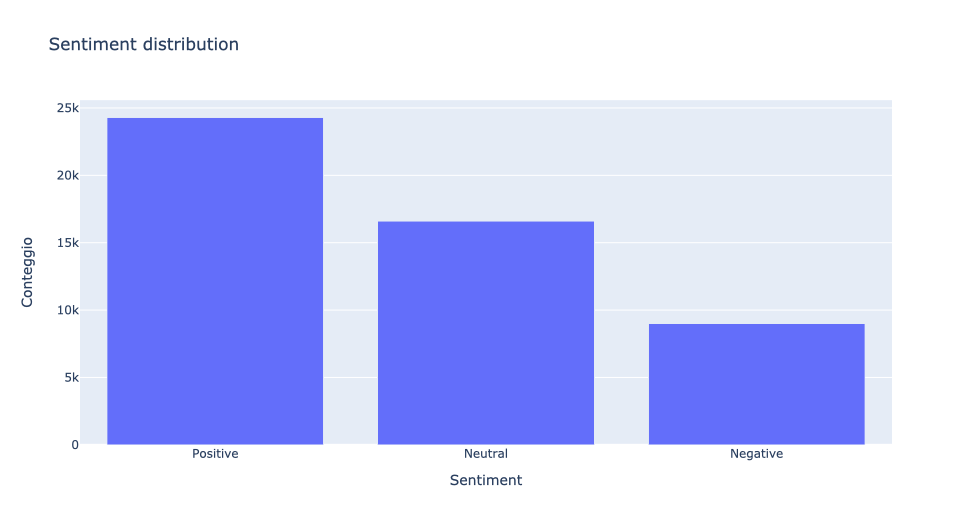
\includegraphics[height=5cm]{sentiment.png}
  \caption{Sentiment analysis about Chat GPT}
  \label{fig:immagine_sentiment}
\end{figure}


\section{Discussion (and Conclusion)}

Lorem ipsum dolor sit amet, consectetur adipiscing elit, sed do eiusmod tempor incididunt ut labore et dolore magna aliqua. Ut enim ad minim veniam, quis nostrud exercitation ullamco laboris nisi ut aliquip ex ea commodo consequat. Duis aute irure dolor in reprehenderit in voluptate velit esse cillum dolore eu fugiat nulla pariatur. Excepteur sint occaecat cupidatat non proident, sunt in culpa qui officia deserunt mollit anim id est laborum.

% The next two lines define the bibliography style to be used, and the bibliography file.
\bibliographystyle{ACM-Reference-Format}
\bibliography{biblio}

\end{document}

